
%% bare_conf.tex
%% V1.4b
%% 2015/08/26
%% by Michael Shell
%% See:
%% http://www.michaelshell.org/
%% for current contact information.
%%
%% This is a skeleton file demonstrating the use of IEEEtran.cls
%% (requires IEEEtran.cls version 1.8b or later) with an IEEE
%% conference paper.
%%
%% Support sites:
%% http://www.michaelshell.org/tex/ieeetran/
%% http://www.ctan.org/pkg/ieeetran
%% and
%% http://www.ieee.org/

%%*************************************************************************
%% Legal Notice:
%% This code is offered as-is without any warranty either expressed or
%% implied; without even the implied warranty of MERCHANTABILITY or
%% FITNESS FOR A PARTICULAR PURPOSE! 
%% User assumes all risk.
%% In no event shall the IEEE or any contributor to this code be liable for
%% any damages or losses, including, but not limited to, incidental,
%% consequential, or any other damages, resulting from the use or misuse
%% of any information contained here.
%%
%% All comments are the opinions of their respective authors and are not
%% necessarily endorsed by the IEEE.
%%
%% This work is distributed under the LaTeX Project Public License (LPPL)
%% ( http://www.latex-project.org/ ) version 1.3, and may be freely used,
%% distributed and modified. A copy of the LPPL, version 1.3, is included
%% in the base LaTeX documentation of all distributions of LaTeX released
%% 2003/12/01 or later.
%% Retain all contribution notices and credits.
%% ** Modified files should be clearly indicated as such, including  **
%% ** renaming them and changing author support contact information. **
%%*************************************************************************


% *** Authors should verify (and, if needed, correct) their LaTeX system  ***
% *** with the testflow diagnostic prior to trusting their LaTeX platform ***
% *** with production work. The IEEE's font choices and paper sizes can   ***
% *** trigger bugs that do not appear when using other class files.       ***                          ***
% The testflow support page is at:
% http://www.michaelshell.org/tex/testflow/



\documentclass[conference]{IEEEtran}
% Some Computer Society conferences also require the compsoc mode option,
% but others use the standard conference format.
%
% If IEEEtran.cls has not been installed into the LaTeX system files,
% manually specify the path to it like:
% \documentclass[conference]{../sty/IEEEtran}





% Some very useful LaTeX packages include:
% (uncomment the ones you want to load)


% *** MISC UTILITY PACKAGES ***
%
%\usepackage{ifpdf}
% Heiko Oberdiek's ifpdf.sty is very useful if you need conditional
% compilation based on whether the output is pdf or dvi.
% usage:
% \ifpdf
%   % pdf code
% \else
%   % dvi code
% \fi
% The latest version of ifpdf.sty can be obtained from:
% http://www.ctan.org/pkg/ifpdf
% Also, note that IEEEtran.cls V1.7 and later provides a builtin
% \ifCLASSINFOpdf conditional that works the same way.
% When switching from latex to pdflatex and vice-versa, the compiler may
% have to be run twice to clear warning/error messages.




% *** CITATION PACKAGES ***
%
\usepackage{cite}
% cite.sty was written by Donald Arseneau
% V1.6 and later of IEEEtran pre-defines the format of the cite.sty package
% \cite{} output to follow that of the IEEE. Loading the cite package will
% result in citation numbers being automatically sorted and properly
% "compressed/ranged". e.g., [1], [9], [2], [7], [5], [6] without using
% cite.sty will become [1], [2], [5]--[7], [9] using cite.sty. cite.sty's
% \cite will automatically add leading space, if needed. Use cite.sty's
% noadjust option (cite.sty V3.8 and later) if you want to turn this off
% such as if a citation ever needs to be enclosed in parenthesis.
% cite.sty is already installed on most LaTeX systems. Be sure and use
% version 5.0 (2009-03-20) and later if using hyperref.sty.
% The latest version can be obtained at:
% http://www.ctan.org/pkg/cite
% The documentation is contained in the cite.sty file itself.






% *** GRAPHICS RELATED PACKAGES ***
%
\ifCLASSINFOpdf
  \usepackage[pdftex]{graphicx}
  % declare the path(s) where your graphic files are
  % \graphicspath{{../pdf/}{../jpeg/}}
  % and their extensions so you won't have to specify these with
  % every instance of \includegraphics
  % \DeclareGraphicsExtensions{.pdf,.jpeg,.png}
\else
  % or other class option (dvipsone, dvipdf, if not using dvips). graphicx
  % will default to the driver specified in the system graphics.cfg if no
  % driver is specified.
  % \usepackage[dvips]{graphicx}
  % declare the path(s) where your graphic files are
  % \graphicspath{{../eps/}}
  % and their extensions so you won't have to specify these with
  % every instance of \includegraphics
  % \DeclareGraphicsExtensions{.eps}
\fi
% graphicx was written by David Carlisle and Sebastian Rahtz. It is
% required if you want graphics, photos, etc. graphicx.sty is already
% installed on most LaTeX systems. The latest version and documentation
% can be obtained at: 
% http://www.ctan.org/pkg/graphicx
% Another good source of documentation is "Using Imported Graphics in
% LaTeX2e" by Keith Reckdahl which can be found at:
% http://www.ctan.org/pkg/epslatex
%
% latex, and pdflatex in dvi mode, support graphics in encapsulated
% postscript (.eps) format. pdflatex in pdf mode supports graphics
% in .pdf, .jpeg, .png and .mps (metapost) formats. Users should ensure
% that all non-photo figures use a vector format (.eps, .pdf, .mps) and
% not a bitmapped formats (.jpeg, .png). The IEEE frowns on bitmapped formats
% which can result in "jaggedy"/blurry rendering of lines and letters as
% well as large increases in file sizes.
%
% You can find documentation about the pdfTeX application at:
% http://www.tug.org/applications/pdftex





% *** MATH PACKAGES ***
%
%\usepackage{amsmath}
% A popular package from the American Mathematical Society that provides
% many useful and powerful commands for dealing with mathematics.
%
% Note that the amsmath package sets \interdisplaylinepenalty to 10000
% thus preventing page breaks from occurring within multiline equations. Use:
%\interdisplaylinepenalty=2500
% after loading amsmath to restore such page breaks as IEEEtran.cls normally
% does. amsmath.sty is already installed on most LaTeX systems. The latest
% version and documentation can be obtained at:
% http://www.ctan.org/pkg/amsmath





% *** SPECIALIZED LIST PACKAGES ***
%
%\usepackage{algorithmic}
% algorithmic.sty was written by Peter Williams and Rogerio Brito.
% This package provides an algorithmic environment fo describing algorithms.
% You can use the algorithmic environment in-text or within a figure
% environment to provide for a floating algorithm. Do NOT use the algorithm
% floating environment provided by algorithm.sty (by the same authors) or
% algorithm2e.sty (by Christophe Fiorio) as the IEEE does not use dedicated
% algorithm float types and packages that provide these will not provide
% correct IEEE style captions. The latest version and documentation of
% algorithmic.sty can be obtained at:
% http://www.ctan.org/pkg/algorithms
% Also of interest may be the (relatively newer and more customizable)
% algorithmicx.sty package by Szasz Janos:
% http://www.ctan.org/pkg/algorithmicx




% *** ALIGNMENT PACKAGES ***
%
%\usepackage{array}
% Frank Mittelbach's and David Carlisle's array.sty patches and improves
% the standard LaTeX2e array and tabular environments to provide better
% appearance and additional user controls. As the default LaTeX2e table
% generation code is lacking to the point of almost being broken with
% respect to the quality of the end results, all users are strongly
% advised to use an enhanced (at the very least that provided by array.sty)
% set of table tools. array.sty is already installed on most systems. The
% latest version and documentation can be obtained at:
% http://www.ctan.org/pkg/array


% IEEEtran contains the IEEEeqnarray family of commands that can be used to
% generate multiline equations as well as matrices, tables, etc., of high
% quality.




% *** SUBFIGURE PACKAGES ***
\ifCLASSOPTIONcompsoc
 \usepackage[caption=false,font=normalsize,labelfont=sf,textfont=sf]{subfig}
\else
  \usepackage[caption=false,font=footnotesize]{subfig}
\fi
% subfig.sty, written by Steven Douglas Cochran, is the modern replacement
% for subfigure.sty, the latter of which is no longer maintained and is
% incompatible with some LaTeX packages including fixltx2e. However,
% subfig.sty requires and automatically loads Axel Sommerfeldt's caption.sty
% which will override IEEEtran.cls' handling of captions and this will result
% in non-IEEE style figure/table captions. To prevent this problem, be sure
% and invoke subfig.sty's "caption=false" package option (available since
% subfig.sty version 1.3, 2005/06/28) as this is will preserve IEEEtran.cls
% handling of captions.
% Note that the Computer Society format requires a larger sans serif font
% than the serif footnote size font used in traditional IEEE formatting
% and thus the need to invoke different subfig.sty package options depending
% on whether compsoc mode has been enabled.
%
% The latest version and documentation of subfig.sty can be obtained at:
% http://www.ctan.org/pkg/subfig




% *** FLOAT PACKAGES ***
%
%\usepackage{fixltx2e}
% fixltx2e, the successor to the earlier fix2col.sty, was written by
% Frank Mittelbach and David Carlisle. This package corrects a few problems
% in the LaTeX2e kernel, the most notable of which is that in current
% LaTeX2e releases, the ordering of single and double column floats is not
% guaranteed to be preserved. Thus, an unpatched LaTeX2e can allow a
% single column figure to be placed prior to an earlier double column
% figure.
% Be aware that LaTeX2e kernels dated 2015 and later have fixltx2e.sty's
% corrections already built into the system in which case a warning will
% be issued if an attempt is made to load fixltx2e.sty as it is no longer
% needed.
% The latest version and documentation can be found at:
% http://www.ctan.org/pkg/fixltx2e


%\usepackage{stfloats}
% stfloats.sty was written by Sigitas Tolusis. This package gives LaTeX2e
% the ability to do double column floats at the bottom of the page as well
% as the top. (e.g., "\begin{figure*}[!b]" is not normally possible in
% LaTeX2e). It also provides a command:
%\fnbelowfloat
% to enable the placement of footnotes below bottom floats (the standard
% LaTeX2e kernel puts them above bottom floats). This is an invasive package
% which rewrites many portions of the LaTeX2e float routines. It may not work
% with other packages that modify the LaTeX2e float routines. The latest
% version and documentation can be obtained at:
% http://www.ctan.org/pkg/stfloats
% Do not use the stfloats baselinefloat ability as the IEEE does not allow
% \baselineskip to stretch. Authors submitting work to the IEEE should note
% that the IEEE rarely uses double column equations and that authors should try
% to avoid such use. Do not be tempted to use the cuted.sty or midfloat.sty
% packages (also by Sigitas Tolusis) as the IEEE does not format its papers in
% such ways.
% Do not attempt to use stfloats with fixltx2e as they are incompatible.
% Instead, use Morten Hogholm'a dblfloatfix which combines the features
% of both fixltx2e and stfloats:
%
% \usepackage{dblfloatfix}
% The latest version can be found at:
% http://www.ctan.org/pkg/dblfloatfix




% *** PDF, URL AND HYPERLINK PACKAGES ***
%
%\usepackage{url}
% url.sty was written by Donald Arseneau. It provides better support for
% handling and breaking URLs. url.sty is already installed on most LaTeX
% systems. The latest version and documentation can be obtained at:
% http://www.ctan.org/pkg/url
% Basically, \url{my_url_here}.




% *** Do not adjust lengths that control margins, column widths, etc. ***
% *** Do not use packages that alter fonts (such as pslatex).         ***
% There should be no need to do such things with IEEEtran.cls V1.6 and later.
% (Unless specifically asked to do so by the journal or conference you plan
% to submit to, of course. )


% correct bad hyphenation here
\hyphenation{op-tical net-works semi-conduc-tor}
\usepackage{amssymb}
\usepackage{amsmath}
\DeclareMathOperator*{\argmin}{arg\,min}
\DeclareMathOperator*{\argmax}{arg\,max}
\usepackage{bbm}


\begin{document}
%
% paper title
% Titles are generally capitalized except for words such as a, an, and, as,
% at, but, by, for, in, nor, of, on, or, the, to and up, which are usually
% not capitalized unless they are the first or last word of the title.
% Linebreaks \\ can be used within to get better formatting as desired.
% Do not put math or special symbols in the title.
\title{Virtual Neurorobotics Practical Report\\Group 5}


% author names and affiliations
% use a multiple column layout for up to three different
% affiliations
\author{\IEEEauthorblockN{Sebastian Monka}
\IEEEauthorblockA{Matriculation number: }
\and

\IEEEauthorblockN{Fabian Peller}
\IEEEauthorblockA{Matriculation number}
\and
\IEEEauthorblockN{Veith R\"othlingsh\"ofer}
\IEEEauthorblockA{Matriculation number: 1764630\\Informatics Master SPO2015}}

% make the title area
\maketitle

% As a general rule, do not put math, special symbols or citations
% in the abstract
\begin{abstract}
In this report, we present our results on the three defined challenges: the perception challenge "Thimblerigger", the motion challenge "Lauron QWOP", and the locomotion challenge "Robotic tennis".
\end{abstract}

% no keywords

\IEEEpeerreviewmaketitle



\section{Introduction}
All experiments run inside the Neurorobotics Platform (NRP) \cite{nrp}. 
The challenges should be solved by utilizing spiking neural networks that are built into the NRP.
Simulations within the NRP are based on the Gazebo simulator \cite{gazebo}.

\section{Perception Challenge}

\subsection{Challenge definition}

The perception challenge is titled "Thimblerigger". An iCUB robot starts in an empty world that contains three red cylinders. A cylinder represents a mug.
One of these mugs contains a green ball underneath. The challenge can reveal which mug contains the ball on request.
The task is to enable the robot to: 
\begin{enumerate}
	\item Find the mug that contains the ball
	\item Track that mug while the mugs are being shuffled
	\item Decide which mug contains the ball after shuffling
\end{enumerate}

Fig.~\ref{fig:challenge} displays the setup of the challenge.

\begin{figure}
	\centering
	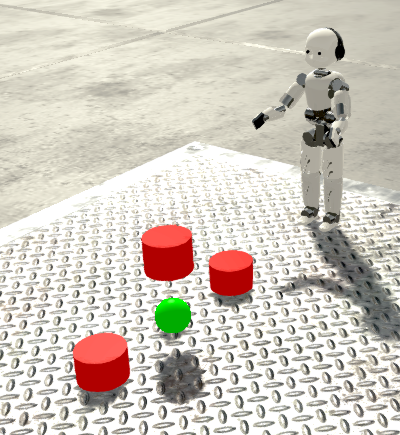
\includegraphics[width=0.4\textwidth]{logos/challenge}
	\caption{The perception challenge environment. The 	second mug is lifted up to display that it contains the 	ball.}
	\label{fig:challenge}
\end{figure}

In the following, we describe approaches to solve the challenge.

\subsection{Working version}
\label{sec:working}
We solve the challenge via a distance-based approach. We move the robot to capture the scene from the side instead of from the front to avoid overlapping mugs in the camera image stream.

We employ four transfer functions to track the ball:
\begin{enumerate}

	\item Track green: Maps the green channel of the input image stream to three neurons $green_i, i\in\{1,2,3\}$. 
	\item Find initial track: Notices once the correct mug is lifted at challenge start by observing the output spikes of  $green_i, i\in\{1,2,3\}$.
	\item Extract centers: Finds the positions of all three mugs in frame $t$ by finding the center points of the three most prominent red contours in the input image stream. For this reason it is important that the mugs do not overlap themselves in the input image stream. The transfer function keeps track of the center point of the predicted mug in frame $t-1$. The prediction is updated based on the closest distance of the previous prediction to the current centers.
	\item Predict: Maps the mug index predicted to contain the ball to one of three $estimate_i,  i\in\{1,2,3\}$ neurons.
\end{enumerate}

All transfer functions requiring image input from the robot camera rely on the stream from the "left eye" camera. Equations~\eqref{eq:distance0} to \eqref{eq:distance10} formalize the tracking mechanism.

In equation~\eqref{eq:distance0}, we define the amplitude of the $green$ neurons  responsible for tracking the green ball to be the mean value of the green channel $g$ in their respective third at time $t$.
\begin{equation}
amplitude(green_{i_t}) = \begin{bmatrix}
           \frac{1}{93}\sum\limits_{y=120}^{160}\sum\limits_{x=85}^{137}g(x+y) \\
           \frac{1}{93}\sum\limits_{y=120}^{160}\sum\limits_{x=138}^{191}g(x+y) \\
           \frac{1}{92}\sum\limits_{y=120}^{160}\sum\limits_{x=192}^{240}g(x+y) \\
         \end{bmatrix}_{i_t}  \label{eq:distance0}
\end{equation}
       
Equations~\eqref{eq:distance2} through \eqref{eq:distance6} describe how the center points of the mugs are extracted from the input image stream. Here, $f$ is a manually tuned threshold function, $r$ is the red channel of the input image, and $b$ is a structuring element defined over $B$ such that $(b \ominus f)$ implements morphological erosion. $C$ is set of $(x,y)$ coordinates of contour center points in the eroded image ordered by their $x$ coordinate.
\begin{align}
f(x) &= \mathbbm{1}\{x >= 150\}\label{eq:distance2}\\
(b \ominus f)(x) &= \inf\limits_{y\in B}[f(x+y)-b(y)]\\
C_{outlines} &= \{c \in contours((b \ominus f)(x)): area(c) > 50\}\\
C &= \{center(c): x \in C_{outlines}\}_{\leq (x,y)}\label{eq:distance6}\\
\end{align}
Finally, $E_{t}$ is the estimated mug index at time $t$. Time $t=0$ is defined to be the moment a $green$ neuron spikes for the first time. The rate of the estimate neuron corresponding to the currently estimated index is set to $100$.
\begin{align}
E_0 &= \argmax\limits_i green_{i_0} \\ 
E_{t} &= \argmin\limits_{i}||C_i - E_{t-1}||_2 \\
rate(estimate_{i, i\in\{1,2,3\}, i\neq E_{t}}) &= 0 \\
rate(estimate_{E_{t}}) &= 100 
\label{eq:distance10}
\end{align}

Using this approach, the challenge is solved close to 100\% of trials. It only fails if a glitch occurs inside the simulator during repositioning of the robot, causing it to fall over. This happens in about $\frac{1}{40}$ of trials and is presumably caused by a race condition inside Gazebo, although this could not be verified.




\subsection{Other approaches}

Two approaches that utilize the spiking neural network to a higher degree have been tested. However, none of them worked to our satisfaction for different reasons. The following paragraphs describe the approaches and why we believe they fail.

\subsubsection*{Neural retina}

A task that is mainly solved using OpenCV~\cite{opencv_library} in the woking version is extraction of the center coordinates of the three mugs. 
We assume that it possible to solve this problem using a neural retina: A grid of $n$ by $m$ neurons that represents the input image. We map the red channel of the camera stream to the retina. The original resolution of the camera stream is $320$ by $240$ pixels, making a one-to-one mapping of pixel-to-neuron computationally challenging. However, the only requirement for the resolution of the retina is sufficient distinction between the different mugs. 
This is achievable with a resolution of $40$ by $30$ neurons, or $\frac{1}{8}$th of each side.

Using an \textit{integrate and fire} model, we arange the neurons' position in the same grid using pyNN's~\cite{pynn} \textit{Space} library and connect neighboring neurons with \begin{enumerate}
\item a static synapse
\item a depressing Tsodyks Markram synapse
\end{enumerate}
We theorize that this connection will focus the highest spiking rate at the center of each mug. To retrieve the current center points of the three mugs, the index of the three neurons with the hightest spiking rate needs to be found.
This approach does not work due to two factors. Firstly, computational power: We run this experiment under a local installation of the NRP under Ubuntu 16.4.3 on a Intel® Core™ i7-6700K CPU @ 4.00GHz x 8, 16 GB RAM and a Nvidia GeForce GTX 1070 8 GB VRAM graphics card, which manages to simulate about one second of time in five minutes of real time. This is infeasible to solve the challenge.
Secondly, no wokring set of synapse and neuron parameters could be found using manual tuning or a random search. 
This manifests itself in the retina: If one neuron spikes, the whole net is overloaded immediately when using depressing Tsodyks Markram synapses. We assume that 
there is a set of parameters that works due to the fading spike characteristic of the depressing synapse (see Fig.~\ref{fig:markram}).

\begin{figure}[!t]
	\centering
	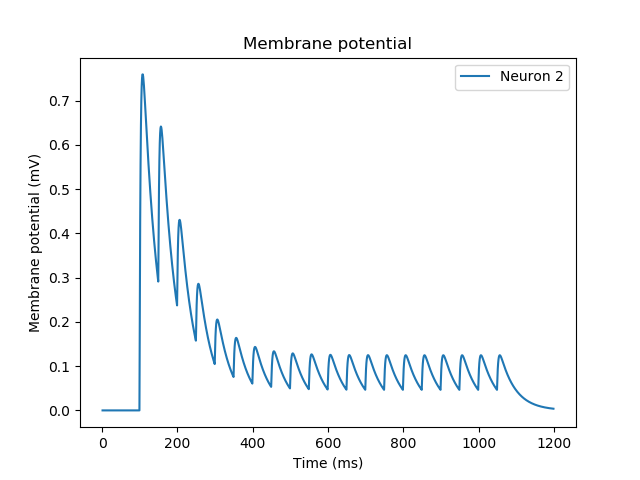
\includegraphics[width=0.4\textwidth]{logos/tsodyks_depressing}
	\caption{The characteristic of a depressing Tsodyks Markram synapse. Source:~\cite{nestweb}}
	\label{fig:markram}
\end{figure}

To increase simulation speed, we also test this setup without connecting the neurons to each other. This significantly improves the frame rate. However, the center points can no longer be found via the retina. We argue that it is not important to find the exact center points, as long as any point on each mug is found.
Due to the implementation of $\argmax$ in the mathematics library \textit{NumPy}~\cite{numpy}, this approach works as long the three mugs are level and the lighing of the scene is in such a way that there is a brightest spot on every mug in the red channel. When this is the case, we are able to identify the location of the three mugs consistently. However, once a mug moves and one is above or below the others in the robot's view, we lose track as neurons belonging to the same mug become "the most active" due to the evaluation order of $\argmax$, which chooses the first instance of the maximal value if there are more than one. To aleviate this problem, we try a neural downsampling technique. An additional layer of neurons half the size of the previous retina layer on every side is added, and $4x4$ neuron patches are connected to one neuron in the next layer. This can be interpreted as a $2x2$ convolution with stride $2$ over the retina. By downsampling with $n$ such layers until every mug corresponds to a single neuron, it possible to find a unique position for each mug. This approach is also limited by computational power, and by the fact that at this point the resolution of the center point coordinates is too small to reliably track them using the distance based approach described in section \ref{sec:working}. See Fig.~\ref{fig:mugs} for a visual description of this process. It could be possible to circumvent this issue by placing the robot further away from the mugs inside the simulation, until the size of one mug corresponds to one neuron in the single-layer retina. Due to time constraints, we were not able to evaluate this hypothesis further.
 

\begin{figure*}[!t]
\centering
\subfloat[Input layer to the neural retina: (thresholded) red color channel of the camera stream.]{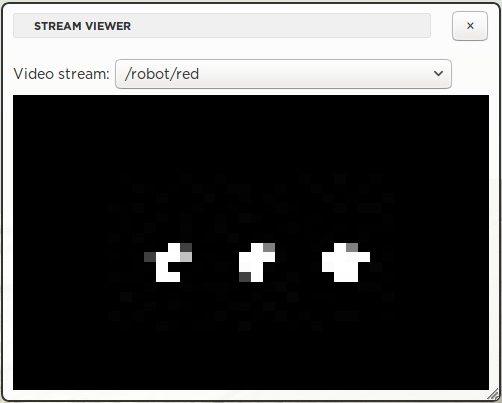
\includegraphics[width=1.5in]{logos/red}%
\label{fig_first_case}}
\hfil
\subfloat[Mugs being detected on the neural retina.]{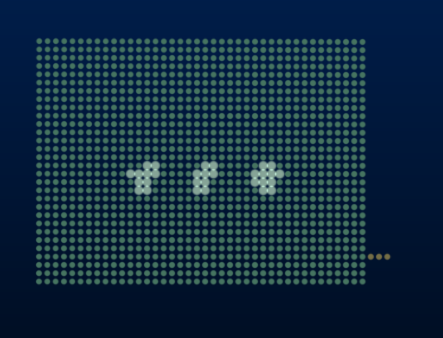
\includegraphics[height=1.2in]{logos/brain2}%
\label{fig_second_case}}
\hfil
\subfloat[Extracted center points from the neural retina. It works in this case due to ideal lighing conditions and the mugs being rooughly level.]{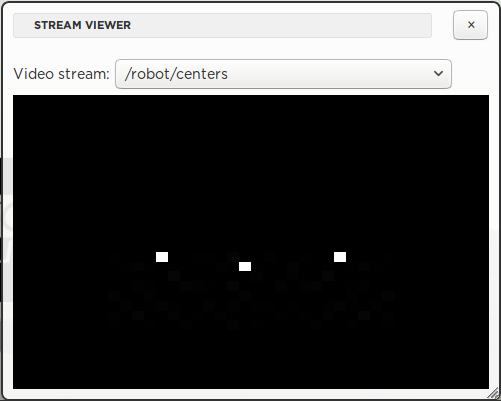
\includegraphics[width=1.5in]{logos/centers}%
\label{fig_third_case}}
\hfil
\subfloat[Downscaling the neural retina by connecting patches of 4 neurons to the next layer.]{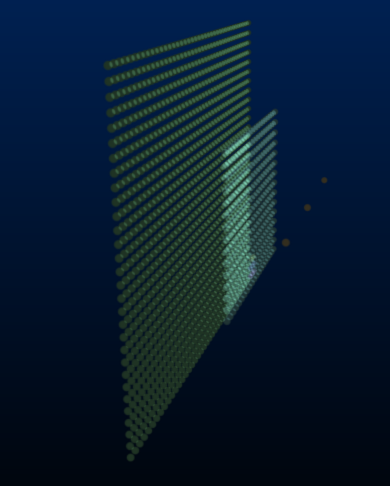
\includegraphics[height=1.2in]{logos/downscale}%
\label{fig_fourth_case}}
\hfil
\caption{Neural retina results}
\label{fig:mugs}
\end{figure*}

%{digraph G {
%rankdir=TB;
%size="6,6"
%ratio = fill;
%node [style=filled];
%"X 1 t" -> "Sum X1" [ label = "exc." color="0.348 0.839 %0.839"];
%"Y 1 t" -> "Sum Y1" [ label = "exc." color="0.348 0.839 %0.839"];
%"X 2 t" -> "Sum X2" [ label = "exc." color="0.348 0.839 0.839"];
%"Y 2 t" -> "Sum Y2" [ label = "exc." color="0.348 0.839 0.839"];
%"X 3 t" -> "Sum X3" [ label = "exc." color="0.348 0.839 %0.839"];
%"Y 3 t" -> "Sum Y3" [ label = "exc." color="0.348 0.839 0.839"];

%"X min t-1" -> "Sum X1" [ label = "inh." color="0.002 0.999 0.999"];
%"X min t-1" -> "Sum X2" [ label = "inh." color="0.002 0.999 0.999"];
%"X min t-1" -> "Sum X3" [ label = "inh." color="0.002 0.999 0.999"];
%"Y min t-1" -> "Sum Y1" [ label = "inh." color="0.002 0.999 0.999"];
%"Y min t-1" -> "Sum Y2" [ label = "inh." color="0.002 0.999 0.999"];
%"Y min t-1" -> "Sum Y3" [ label = "inh." color="0.002 0.999 0.999"];

%"Sum X1" -> "Norm 1" [ label = "exc." color="0.348 0.839 0.839"];
%"Sum Y1" -> "Norm 1" [ label = "exc." color="0.348 0.839 0.839"];
%"Sum X2" -> "Norm 2" [ label = "exc." color="0.348 0.839 0.839"];
%"Sum Y2" -> "Norm 2" [ label = "exc." color="0.348 0.839 0.839"];
%"Sum X3" -> "Norm 3" [ label = "exc." color="0.348 0.839 0.839"];
%"Sum Y3" -> "Norm 3" [ label = "exc." color="0.348 0.839 0.839"];
%}}%
\subsubsection*{Neural norm}

\section{Motion Challenge}

\section{Locomotion Challenge}


% An example of a floating figure using the graphicx package.
% Note that \label must occur AFTER (or within) \caption.
% For figures, \caption should occur after the \includegraphics.
% Note that IEEEtran v1.7 and later has special internal code that
% is designed to preserve the operation of \label within \caption
% even when the captionsoff option is in effect. However, because
% of issues like this, it may be the safest practice to put all your
% \label just after \caption rather than within \caption{}.
%
% Reminder: the "draftcls" or "draftclsnofoot", not "draft", class
% option should be used if it is desired that the figures are to be
% displayed while in draft mode.
%
%\begin{figure}[!t]
%\centering
%\includegraphics[width=2.5in]{myfigure}
% where an .eps filename suffix will be assumed under latex, 
% and a .pdf suffix will be assumed for pdflatex; or what has been declared
% via \DeclareGraphicsExtensions.
%\caption{Simulation results for the network.}
%\label{fig_sim}
%\end{figure}

% Note that the IEEE typically puts floats only at the top, even when this
% results in a large percentage of a column being occupied by floats.


% An example of a double column floating figure using two subfigures.
% (The subfig.sty package must be loaded for this to work.)
% The subfigure \label commands are set within each subfloat command,
% and the \label for the overall figure must come after \caption.
% \hfil is used as a separator to get equal spacing.
% Watch out that the combined width of all the subfigures on a 
% line do not exceed the text width or a line break will occur.
%
%\begin{figure*}[!t]
%\centering
%\subfloat[Case I]{\includegraphics[width=2.5in]{box}%
%\label{fig_first_case}}
%\hfil
%\subfloat[Case II]{\includegraphics[width=2.5in]{box}%
%\label{fig_second_case}}
%\caption{Simulation results for the network.}
%\label{fig_sim}
%\end{figure*}
%
% Note that often IEEE papers with subfigures do not employ subfigure
% captions (using the optional argument to \subfloat[]), but instead will
% reference/describe all of them (a), (b), etc., within the main caption.
% Be aware that for subfig.sty to generate the (a), (b), etc., subfigure
% labels, the optional argument to \subfloat must be present. If a
% subcaption is not desired, just leave its contents blank,
% e.g., \subfloat[].


% An example of a floating table. Note that, for IEEE style tables, the
% \caption command should come BEFORE the table and, given that table
% captions serve much like titles, are usually capitalized except for words
% such as a, an, and, as, at, but, by, for, in, nor, of, on, or, the, to
% and up, which are usually not capitalized unless they are the first or
% last word of the caption. Table text will default to \footnotesize as
% the IEEE normally uses this smaller font for tables.
% The \label must come after \caption as always.
%
%\begin{table}[!t]
%% increase table row spacing, adjust to taste
%\renewcommand{\arraystretch}{1.3}
% if using array.sty, it might be a good idea to tweak the value of
% \extrarowheight as needed to properly center the text within the cells
%\caption{An Example of a Table}
%\label{table_example}
%\centering
%% Some packages, such as MDW tools, offer better commands for making tables
%% than the plain LaTeX2e tabular which is used here.
%\begin{tabular}{|c||c|}
%\hline
%One & Two\\
%\hline
%Three & Four\\
%\hline
%\end{tabular}
%\end{table}


% Note that the IEEE does not put floats in the very first column
% - or typically anywhere on the first page for that matter. Also,
% in-text middle ("here") positioning is typically not used, but it
% is allowed and encouraged for Computer Society conferences (but
% not Computer Society journals). Most IEEE journals/conferences use
% top floats exclusively. 
% Note that, LaTeX2e, unlike IEEE journals/conferences, places
% footnotes above bottom floats. This can be corrected via the
% \fnbelowfloat command of the stfloats package.




\section{Conclusion}
The conclusion goes here.







% trigger a \newpage just before the given reference
% number - used to balance the columns on the last page
% adjust value as needed - may need to be readjusted if
% the document is modified later
%\IEEEtriggeratref{8}
% The "triggered" command can be changed if desired:
%\IEEEtriggercmd{\enlargethispage{-5in}}

% references section

% can use a bibliography generated by BibTeX as a .bbl file
% BibTeX documentation can be easily obtained at:
% http://mirror.ctan.org/biblio/bibtex/contrib/doc/
% The IEEEtran BibTeX style support page is at:
% http://www.michaelshell.org/tex/ieeetran/bibtex/
%\bibliographystyle{IEEEtran}
% argument is your BibTeX string definitions and bibliography database(s)
%\bibliography{IEEEabrv,../bib/paper}
%
% <OR> manually copy in the resultant .bbl file
% set second argument of \begin to the number of references
% (used to reserve space for the reference number labels box)
\bibliographystyle{IEEEtran}
\bibliography{references}



% that's all folks
\end{document}


